%-----------------------------------------------------------------
% TITLE PAGE
%-----------------------------------------------------------------
	% deactivate header and footer
	\pagestyle{superempty}
	
    % creates title blocks
	\fronttitleprep{
        \resizebox{10cm}{!}{\titlefont\textbf{\colorbox{color1}{\textcolor{white}{\aircraftlong}}}}
    }{
        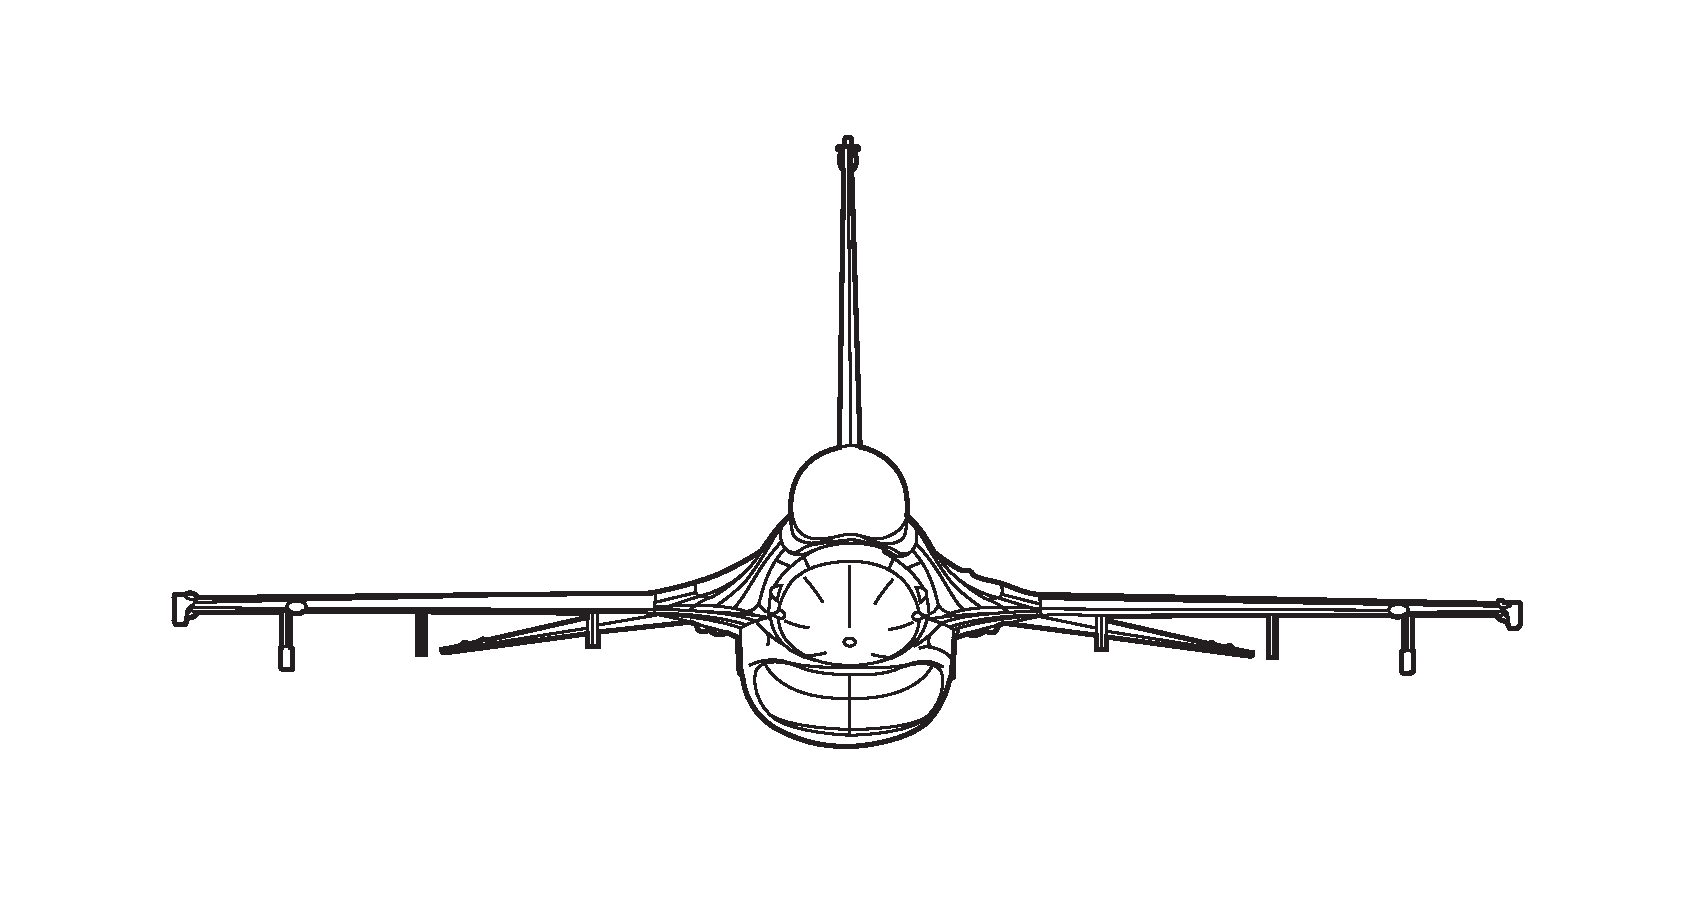
\includegraphics[
            width=0.95\linewidth
        ]{F16_Front.pdf}
    }
	
	% label for hyperrefs back to frontpage
	\label{frontpage}
	% make chevrons
    % use tabular for multi line node
	\thumbfront{Procedures}{0}
	\thumbfront{Systems}{1}
	\thumbfront{\begin{tabular}{c} APG-68 \\ FCR \end{tabular}}{2} 
	\thumbfront{\begin{tabular}{c} TGP / HTS \\ HMD / DL \end{tabular}}{3}
	\thumbfront{\begin{tabular}{c} A/G \\ Weapons \end{tabular}}{4}
	\thumbfront{\begin{tabular}{c} A/A \\ Weapons \end{tabular}}{5}
	\thumbfront{Appendix}{6}
	\thumbwide

	\clearpage
	
	\null\vspace{0cm}

	\begin{tcolorbox}[
		enhanced, colback=white, colframe=color1, colbacktitle=white, coltitle=color1, sharp corners, attach boxed title to top center={yshift=2mm},
		boxed title style={
			sharp corners,
			drop shadow=color1!100
		}, title=\LARGE\textbf{DISCLAIMER}
	]
		\textbf{This document represents a personal project and is intended for entertainment purposes only. Do not use for training purposes or in real life scenarios.}
	\end{tcolorbox}
    
    \vspace{1cm}

    \notebox{
        \cbstart
        \begin{description}
            \item[Obligatory Steps] --
            Solid bars along the page edge signify that the corresponding information is not optional. 
            Procedural steps marked as such can not be skipped without impacting mission capability signficantly.

            \item[Warning] -- this does \textbf{not} mean that all information which is not marked is therefore optional.
        \end{description}
        \cbend
    }

	\cleardoublepage
